%\documentclass[10pt,aspectratio=169]{beamer}
\documentclass[10pt,aspectratio=169,handout]{beamer}

\usetheme{Boadilla}
\usepackage[utf8]{inputenc}
\usepackage[T1]{fontenc}
\usepackage{lmodern}
\usepackage{lipsum}
\usetheme{default}
\usepackage{listings}
\usepackage{hyperref}
\hypersetup{
	colorlinks=true,
	linkcolor=blue,
	filecolor=magenta,      
	urlcolor=cyan
}
\lstset{language=[90]Fortran,
	basicstyle=\small\ttfamily,
	showtabs=false,
	tabsize=2,      
	keywordstyle=\color{red},
	commentstyle=\color{green},
	morecomment=[l]{!\ }% Comment only with space after !
}

%%%%%%%%%%%%%GTA
%\renewcommand{\(}{\left(}
%\renewcommand{\)}{\right)}
%\renewcommand{\[}{\left[}
%\renewcommand{\]}{\right]}

\newcommand{\calpha}{\alpha^\ast}
\newcommand{\calphas}{\alpha^{\ast2}}
\newcommand{\Kr}[2]{\delta_{#1}^{#2}}

%%%%%%%%%%%%%%%%%%%%


\newcommand{\sqNsotwo}{\sqrt{\dfrac{Ns}{2}}}
\newcommand{\oneoNs}{\dfrac{1}{Ns}}

\let\originalleft\left
\let\originalright\right
\renewcommand{\left}{\mathopen{}\mathclose\bgroup\originalleft}
\renewcommand{\right}{\aftergroup\egroup\originalright}


\newcommand{\vect}[1]{\boldsymbol{#1}}
\renewcommand{\vec}[1]{\vect{#1}}

\makeatletter
\newcommand*\bigcdot{{\color{gray}\mathpalette\bigcdot@{1.}}}
\newcommand*\bigcdot@[2]{\mathbin{\vcenter{\hbox{\scalebox{#2}{$\m@th#1\bullet$}}}}}
\makeatother


\DeclareMathOperator*{\argmax}{argmax}
\DeclareMathOperator*{\argmin}{argmin}
\def\rme{{\rm {e}}}
\def\rmi{{\rm {i}}}
\renewcommand{\d}{{\rm {d}}}
\def\dt{{\rm {d}}t}
\def\dddt{\dfrac{\d}{\dt}}
\def\ddt{\frac{\d}{\dt}}

% \newcommand{\sgn}{\mathop{\mathrm{sgn}}}

\newcommand{\diag}{\mathrm{diag}}


\newcommand{\idhat}{\hat{\mathds{1}}}
\newcommand{\id}{\mathds{1}}
\newcommand{\idres}{\id_\mathrm{res}}
\newcommand{\idsys}{\id_\mathrm{sys}}

\newcommand{\trfrak}{\mathfrak{Tr}}
\def\tr{{\rm{Tr}}}
\newcommand{\abss}[1]{\left|#1\right|^2}
\newcommand{\mean}[1]{\left\langle #1 \right\rangle}
\newcommand{\expect}[1]{\mathbb{E}\left[ #1\right]}

%%%%%%%%%%%%%%%%%%% units
\newcommand{\micron}{\rm{\si{\micro\meter}}}


%%%%%%%%%%%%%%%%%%% Greek letters

\newcommand{\alphatil}{{\Tilde{\alpha}}}
\newcommand{\ass}{\alpha_{\mathrm{SS}}}
\newcommand{\alphass}{\alpha_\mathrm{SS}}
\newcommand{\alphahat}{\hat{\alpha}}
\newcommand{\betahat}{\hat{\beta}}
\newcommand{\betatil}{{\Tilde{\beta}}}
% \newcommand{\betatil}{\Tilde{\beta}}

\newcommand{\delhat}{\hat{\delta}}
\newcommand{\ddelhat}{\hat{\delta}^\dagger}

\newcommand{\Jhat}{\hat{J}}

\newcommand{\Lammat}{\boldsymbol{\Lambda}}

\newcommand{\lambdown}{\lambda^{\downarrow}}

\newcommand{\rhoh}{\hat{\rho}}

\newcommand{\rhohat}{\hat{\rho}}
\newcommand{\rhotil}{\tilde{\rho}}
\newcommand{\rhoss}{\rhohat_{\mathrm{SS}}}

\newcommand{\phihat}{\hat{\phi}}
\newcommand{\phidot}{\Dot{\phi}}
\newcommand{\phimat}{\vec{\Phi}}

\newcommand{\Pihat}{\hat{\Pi}}
\newcommand{\pihat}{\hat{\pi}}
\newcommand{\piit}{\mathit{\Pi}}
\newcommand{\piithat}{\hat{\piit}}

\newcommand{\psitilde}{\widetilde{\ket{\psi}}}

\newcommand{\epsvec}{\vec{\epsilon}}

\newcommand{\Obold}{\mathbf{\Omega}}

\newcommand{\Gammatil}{\Tilde{\Gamma}}

\newcommand{\sigmam}{\hat{\sigma}^{-}}
\newcommand{\sigmap}{\hat{\sigma}^{+}}
\newcommand{\sigmax}{\hat{\sigma}^{x}}
\newcommand{\sigmay}{\hat{\sigma}^{y}}
\newcommand{\sigmaz}{\hat{\sigma}^{z}}
\newcommand{\sigmamz}{\hat{\sigma}^{-z}}
\newcommand{\sigmamx}{\hat{\sigma}^{-x}}

\newcommand{\ssp}{\hat{\sigma}^+}
\newcommand{\ssm}{\hat{\sigma}^-}
\newcommand{\ssx}{\hat{\sigma}^x}
\newcommand{\ssy}{\hat{\sigma}^y}
\newcommand{\ssz}{\hat{\sigma}^z}
\newcommand{\ssa}{\hat{\sigma}^\alpha}
\newcommand{\sssz}{\hat{\sigma}^z}
\newcommand{\sigbold}{\bm{\sigma}}

\newcommand{\sigmahat}{\hat{\sigma}}

%%%%%%%%%%%%%%%% abbreviations
\newcommand{\schr}{Schr\"{o}dinger}
\newcommand{\kg}{{\mathrm{KG}}}

\newcommand{\hc}{\mathrm{H.c.}}
%\newcommand{\pv}{\mathrm{p.v.}}

\newcommand{\LP}{\mathrm{LP}}
\newcommand{\UP}{\mathrm{UP}}

%%%%%%%%%%%%%%%% Latin letters


\newcommand{\aaa}{\hat{a}}
\newcommand{\daaa}{\hat{a}^\dagger}
\newcommand{\daaas}{\hat{a}^{\dagger 2}}
\newcommand{\aaas}{\aaa^{2}}

\newcommand{\Ahat}{\hat{A}}
\newcommand{\dAhat}{\Ahat^{\dagger}}
\newcommand{\Atil}{\hat{\tilde{A}}}
\newcommand{\dAtil}{\hat{\tilde{A}}^\dagger}


\newcommand{\Avec}{\vec{A}}
\newcommand{\Avechat}{\hat{\bm{A}}}
\newcommand{\acal}{\mathcal{A}}

\newcommand{\bbb}{\hat{b}}
\newcommand{\dbbb}{\hat{b}^\dagger}
\newcommand{\bbbs}{\bbb^{2}}
\newcommand{\dbbbs}{\bbb^{\dagger 2}}

\newcommand{\BS}{\widehat{\mathrm{BS}}}

\newcommand{\bvec}{\vec{b}}

\newcommand{\Bvec}{\vec{B}}
\newcommand{\Bvechat}{\hat{\bm{B}}}

\newcommand{\Bhat}{\hat{B}}

\newcommand{\cvec}{\vec{c}}
% \newcommand{\ccal}{\mathcal{C}}
\newcommand{\ccc}{\hat{c}}
\newcommand{\dccc}{\hat{c}^\dagger}

\newcommand{\ccal}{\mathcal{C}}

\newcommand{\dcal}{\mathcal{D}}

\newcommand{\dvec}{\vec{d}}

\newcommand{\Ehat}{\hat{E}}
\newcommand{\Evec}{\vec{E}}
\newcommand{\evec}{\vec{e}}
\newcommand{\Evechat}{\hat{\bm{E}}}
\newcommand{\ecal}{\mathcal{E}}



\newcommand{\Fbold}{\mathbf{F}}

\newcommand{\fhat}{\hat{f}}
\newcommand{\fcal}{\mathcal{F}}
\newcommand{\gcal}{\mathcal{G}}
\newcommand{\Gmat}{\boldsymbol{\mathrm{G}}}

% \newcommand{\Ehat}{\hat{E}}
\newcommand{\ecalf}{\ecal^{F}}

\newcommand{\ecalu}{\ecal^{U}}
\newcommand{\fcalu}{\fcal^{U}}
\newcommand{\czu}{\ccal_{\ztil}^{U}}

\newcommand{\ecaluc}{\ecal^{U*}}
\newcommand{\fcaluc}{\fcal^{U*}}
\newcommand{\czuc}{\ccal_{\ztil}^{U*}}

\newcommand{\ecald}{\ecal^{D}}
\newcommand{\fcald}{\fcal^{D}}
\newcommand{\czd}{\ccal_{\ztil}^{D}}

\newcommand{\ecaldc}{\ecal^{D*}}
\newcommand{\fcaldc}{\fcal^{D*}}
\newcommand{\czdc}{\ccal_{\ztil}^{D*}}

\newcommand{\ecali}{\ecal^{I}}
\newcommand{\fcali}{\fcal^{I}}
\newcommand{\czi}{\ccal_{\ztil}^{I}}

\newcommand{\ecalic}{\ecal^{I*}}
\newcommand{\fcalic}{\fcal^{I*}}
\newcommand{\czic}{\ccal_{\ztil}^{I*}}


\newcommand{\hcal}{\mathcal{H}}
\newcommand{\hh}{\hat{H}}
\newcommand{\heff}{\hat{H}_\text{eff}}

\newcommand{\Hhat}{\hat{H}}
\newcommand{\hhat}{\hat{h}}
\newcommand{\htil}{\tilde{H}}

\newcommand{\Khat}{\hat{K}}
\newcommand{\kvec}{{\vec{k}}}


\newcommand{\lio}{\mathcal{L}}
\newcommand{\liou}{\mathcal{L}}
\newcommand{\Liou}{\liou}

\newcommand{\lioeff}{\mathcal{L}_\text{eff}}

\newcommand{\lcal}{\mathcal{L}}
\newcommand{\Lhat}{\hat{L}}
\newcommand{\Ltil}{\tilde{L}}
\newcommand{\Lcal}{\mathcal{L}}

\newcommand{\mev}{\mathrm{meV}}


\newcommand{\mcal}{\mathcal{M}}

\newcommand{\mvec}{{\vec{m}}}
\newcommand{\nsys}{{N_\mathrm{sys}}}
\newcommand{\nres}{{N_\mathrm{res}}}

\newcommand{\ncal}{\mathcal{N}}

\newcommand{\nvec}{{\vec{n}}}

\newcommand{\ohat}{\hat{O}}
\newcommand{\otil}{\tilde{O}}
\newcommand{\ovec}{{\vec{0}}}
\newcommand{\ocal}{\mathcal{O}}

\newcommand{\Ohat}{\hat{O}}

\newcommand{\phat}{\hat{p}}
\newcommand{\pvec}{\vec{p}}
\newcommand{\pcal}{\mathcal{P}}
\newcommand{\pscr}{{\mathscr{P}}}

\newcommand{\qdot}{\dot{q}}
\newcommand{\qhat}{\hat{q}}
\newcommand{\qvec}{\vec{q}}
\newcommand{\qcal}{\mathcal{Q}}
\newcommand{\Rhat}{\hat{R}}
\newcommand{\Rtil}{\tilde{R}}

\newcommand{\R}{\mathbb{R}}

\newcommand{\rvec}{\vec{r}}
\newcommand{\res}{\mathrm{res}}

\newcommand{\rf}{{\mathrm{RF}}}

\newcommand{\Shat}{\hat{S}}
\newcommand{\shat}{\hat{s}}
\newcommand{\svec}{\hat{\vec{\sigma}}}
\newcommand{\sys}{\mathrm{sys}}

\newcommand{\Svec}{\vec{S}}
\newcommand{\Stil}{\tilde{S}}
\newcommand{\Sbold}{\mathbf{S}}
\newcommand{\scal}{\mathcal{S}}

\newcommand{\tcal}{\mathcal{T}}

\newcommand{\Uhat}{\uhat}
\newcommand{\uhat}{\hat{U}}
\newcommand{\udag}{\hat{U}^\dagger}
\newcommand{\Umat}{\boldsymbol{\mathrm{U}}}
\newcommand{\uvec}{\vec{u}}

\newcommand{\ua}{u^{(a)}}
\newcommand{\uac}{u^{(a)*}}
\newcommand{\uab}{u^{(ab)}}
\newcommand{\uabc}{u^{(ab)*}}
\newcommand{\ub}{u^{(b)}}
\newcommand{\ubc}{u^{(b)*}}




\newcommand{\delhata}{\hat{\delta}^{(a)}}
\newcommand{\delhatb}{\hat{\delta}^{(b)}}

\newcommand{\ddelhata}{\hat{\delta}^{(a)\dagger}}
\newcommand{\ddelhatb}{\hat{\delta}^{(b)\dagger}}

\newcommand{\wvec}{\vec{w}}

\newcommand{\xhat}{\hat{x}}

\newcommand{\xvec}{\vec{x}}
\newcommand{\xmu}{x^{\mu}}
\newcommand{\xpmu}{x^{\prime\mu}}
\newcommand{\xnu}{x^{\nu}}
\newcommand{\xpnu}{x^{\prime\nu}}

\newcommand{\rmx}{\mathrm{x}}
\newcommand{\xvecrm}{\vec{\mathrm{x}}}
\newcommand{\rmxvec}{\xvecrm}
\newcommand{\Xvec}{\vec{X}}
\newcommand{\xcal}{\mathcal{X}}

\newcommand{\xtil}{{\Tilde{x}}}

\newcommand{\yvec}{\vec{y}}
\newcommand{\ycal}{\mathcal{Y}}
\newcommand{\ytil}{{\Tilde{y}}}

\newcommand{\Vhat}{\hat{V}}
\newcommand{\ztil}{{\Tilde{z}}}
\newcommand{\z}{\mathbb{Z}}
\newcommand{\zerovec}{\vec{0}}
\newcommand{\zvec}{{\vec{z}}}

\newcommand{\zcal}{\mathcal{Z}}
% \renewcommand{\ket}[1]{|#1\rangle}

\newcommand{\pmx}[1]{\begin{pmatrix}
		#1
\end{pmatrix}}


\newcommand{\bea}{\begin{equation*}\begin{aligned}}
		\newcommand{\eea}{\end{aligned}\end{equation*}}
\newcommand{\be}{\begin{equation*}}
	\newcommand{\ee}{\end{equation*}}

\newcommand{\redtext}[1]{\textcolor{red}{#1}}

\begin{document}
\author{Zejian Li \\(li.zejian@ictp.it)}
\title{Lecture 1: Linear Regression}
\subtitle{with least-squares fitting}
%\logo{}
%\institute{}
\date{16 Oct. 2024}
%\subject{}
%\setbeamercovered{transparent}
%\setbeamertemplate{navigation symbols}{}


% ----------------------------------------------------------------
\begin{frame}[plain]
	\maketitle
\end{frame}


% ----------------------------------------------------------------
\section{Introduction}

\begin{frame}
	\frametitle{Curve fitting - Introduction}
	The process of constructing a parametrized function $f(\vec{x}; \vec{\beta})$ that has the best fit to a series of data points $\{(\vec{x}_i,y_i)\}_i$. \\ \pause
	
	\vspace{0.5pt}
	For example...
	\vspace{-0.5cm}
	\begin{columns}[t]
	\column{0.5\textwidth}
		\begin{itemize}[<+->]
		\item Linear regression:
		\bea
		f(x;\beta_1,\beta_2) = \beta_1 + \beta_2 x
		\eea
		\end{itemize}
		\begin{figure}
			\centering
			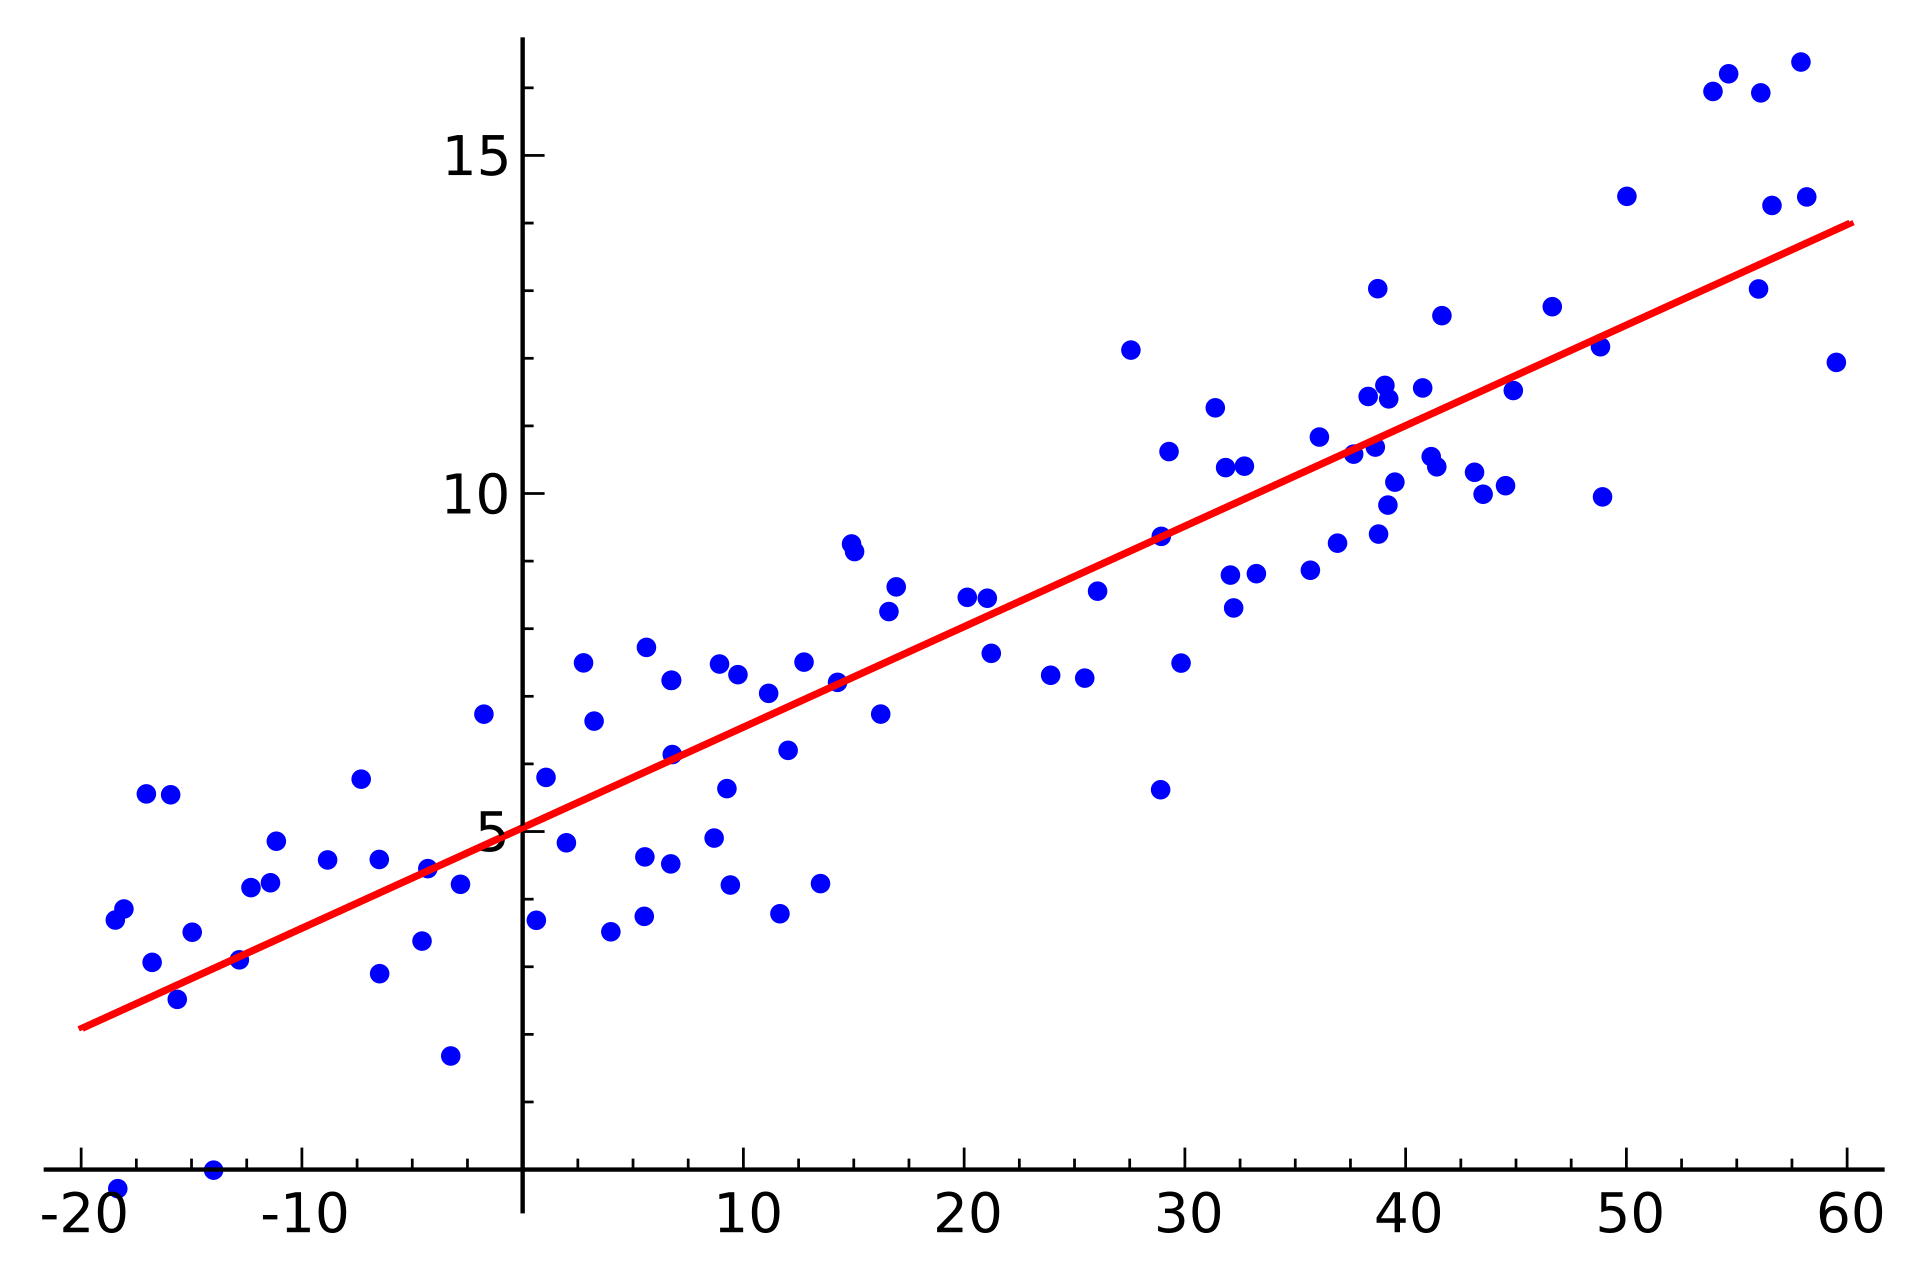
\includegraphics[width=0.8\textwidth]{fig/Linear_regression.svg.png}
		\end{figure}%

		\column{0.5\textwidth}
		\begin{itemize}[<+->]
			
			\item Training an AI (supervised learning):\\
			$f(\vec{x};\vec{\beta})$ is an complicated nonlinear function (often represented as a ``neural network'') that can be trained (optimizing the parameters $\vec{\beta}$) to learn patterns in the input $\vec{x}$.
			
			\begin{figure}
				\centering
				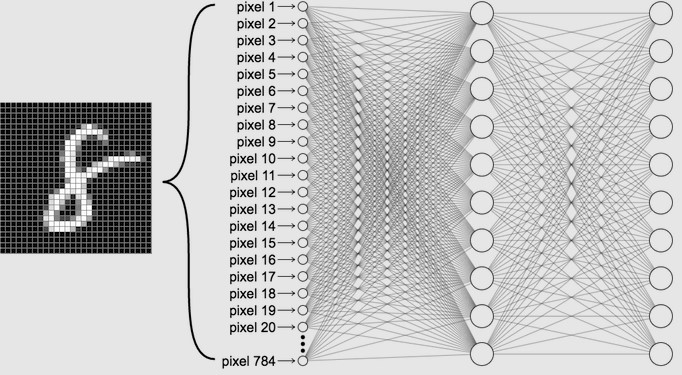
\includegraphics[width=0.8\textwidth]{fig/ann}
			\end{figure}%
		\end{itemize}
		\end{columns}

\end{frame}



\begin{frame}{Curve (over-)fitting }
	\begin{columns}
		\column{0.3\textwidth}
			``With four parameters I can fit an elephant, and with five I can make him wiggle his trunk.''\\
			\quad \quad --- John von Neumann
		\column{0.5\textwidth}
		\begin{figure}
			\centering
			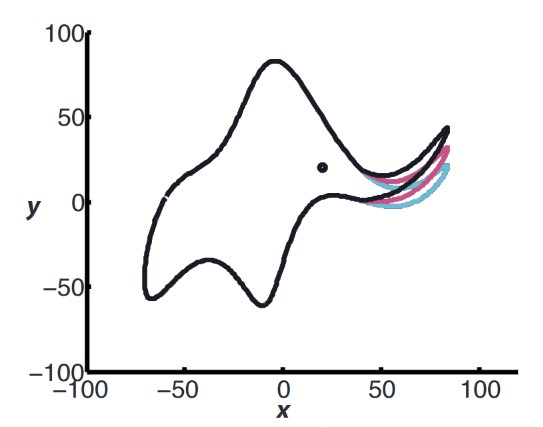
\includegraphics[width=0.8\textwidth]{fig/elephant}
		\end{figure}%
	\begin{center}
	 The Fermi-Neumann elephant. \\ (See \href{https://doi.org/10.1119/1.3254017}{Am. J. Phys. 1 June 2010; 78 (6): 648–649})
	\end{center}

	\end{columns}
\end{frame}

\begin{frame}{Linear least-squares fitting}
	The procedure for fitting a {\color{blue}linear function} by minimizing the {\color{blue} sum of the squares of the residuals} of the points from the curve.
	\begin{columns}
		\column{0.6\textwidth}
			\begin{itemize}[<+->]
				\item Input: dataset with $N$ points $\{(x_1,y_1),...,(x_N,y_N)\}$.
				\item Assumption: errors $\varepsilon_i$ are only in $y_i$,
				\bea
					y_i = f(x_i) + \varepsilon_i\,,
				\eea
				and are normally distributed $\varepsilon\sim \ncal(0,\sigma^2\mathbb{I})$.
				\item Linear model (the function we want to fit): 
				\bea
					f(x;\beta_1,\beta_2) = \beta_1+\beta_2 x\,.
				\eea
				\item Sum of squared residuals (the quantity to be minimized):
				\bea
					S_\mathrm{res} &\equiv \sum_i [y_i - f(x_i)]^2 \\
					&= \sum_i [y_i - (\beta_1 + \beta_2 x_i)]^2\,.
				\eea
			\end{itemize}
		
		\column{0.3\textwidth}
		\begin{figure}
			\centering
			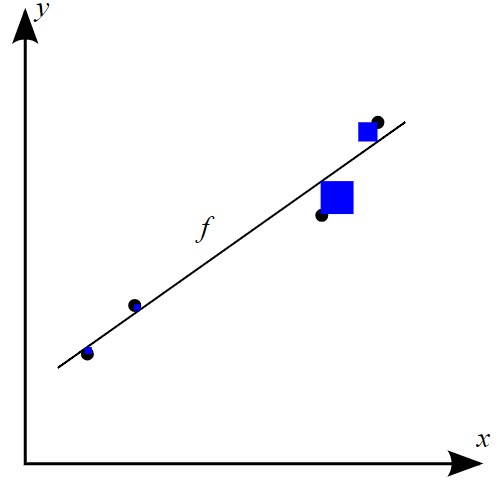
\includegraphics[width=0.9\textwidth]{fig/sres}
		\end{figure}
	\begin{center}
		Squares of residuals
	\end{center}
	\end{columns}
\end{frame}

\begin{frame}{Linear least-squares fitting}
We now minimize the sum of squared residuals:
	\bea
	S_\mathrm{res}(\beta_1,\beta_2) &\equiv \sum_i [y_i - f(x_i)]^2 = \sum_i [y_i - (\beta_1 + \beta_2 x_i)]^2\,.
	\eea
	\vspace{-0.5cm}\pause
	\begin{itemize}[<+->]
	\item We require the partial derivatives $\partial_{\vec{\beta}} S_\mathrm{res}$ to be zero at the minimum:
	\bea
		\dfrac{\partial S_\mathrm{res}}{\partial \beta_1} &= -2\sum_{i=1}^N [y_i - \beta_1 - \beta_2 x_i] = 0\,,\\
		\dfrac{\partial S_\mathrm{res}}{\partial \beta_2} &= -2\sum_{i=1}^N [y_i - \beta_1 - \beta_2 x_i] x_i = 0\,.
	\eea
	\item This is a linear system for $(\beta_1,\beta_2)$ that you know how to solve with Cramer's rule (see last lecture):
	\bea
		\begin{bmatrix}
			N & \Sigma_i x_i \\
			\Sigma_i x_i & \Sigma_i x_i^2
		\end{bmatrix}
	\begin{bmatrix}
		\beta_1 \\ \beta_2
	\end{bmatrix}
  = 
  \begin{bmatrix}
  	\Sigma_i y_i \\ \Sigma_i x_i y_i
  \end{bmatrix}\quad\longrightarrow \quad\begin{bmatrix}
  \betahat_1 \\ \betahat_2
\end{bmatrix}
= 		\begin{bmatrix}
N & \Sigma_i x_i \\
\Sigma_i x_i & \Sigma_i x_i^2
\end{bmatrix}^{-1}
\begin{bmatrix}
\Sigma_i y_i \\ \Sigma_i x_i y_i
\end{bmatrix}\,,
	\eea
\item Estimator for the fit function: $\fhat(x) \equiv f(x;\betahat_1,\betahat_2)$.
	
\end{itemize}
\end{frame}

\begin{frame}{Quality of the fit and error estimation}
	\begin{itemize}
		\item Overall quality of the fit: coefficient of determination $R^2$:
		\bea
			R^2 \equiv 1 - \dfrac{{\color{blue}S_\mathrm{res}}}{{\color{red}S_\mathrm{tot}}}\,,\quad  {\color{red}S_\mathrm{tot}}\equiv \sum_i (y_i - \overline{y})^2\,,\quad {\color{blue} S_\mathrm{res}} \equiv \sum_i [y_i - \fhat(x_i)]^2\,,\quad \overline{y} \equiv \dfrac{1}{N}\sum_{i=1}^N y_i\,.
		\eea
	\end{itemize}
\begin{figure}
	\centering
	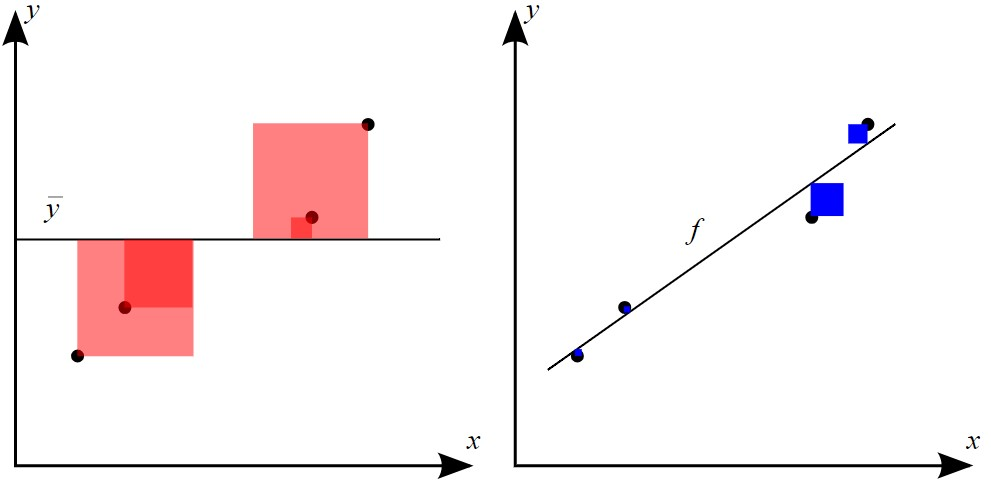
\includegraphics[width=0.5\textwidth]{fig/rsq}
\end{figure}
\end{frame}


\begin{frame}{Quality of the fit and error estimation}
	\begin{itemize}[<+->]
		\item Overall quality of the fit: coefficient of determination $R^2$:
		\bea
		R^2 \equiv 1 - \dfrac{{\color{blue}S_\mathrm{res}}}{{\color{red}S_\mathrm{tot}}}\,,\quad  {\color{red}S_\mathrm{tot}}\equiv \sum_i (y_i - \overline{y})^2\,,\quad {\color{blue} S_\mathrm{res}} = \sum_i [y_i - \fhat(x_i)]^2\,,\quad \overline{y} = \dfrac{1}{N}\sum_{i=1}^N y_i\,.
		\eea
		\item Estimator for the variance $\sigma^2$ of the error $\varepsilon_i = y_i - f(x_i)$:
		\bea
		\sigmahat^2 = \sum_{i = 1}^N\dfrac{\varepsilon_i^2}{N-2}\,.
		\eea
		\item Standard errors (SE) for the fit parameters:
		\bea
			\widehat{\mathrm{SE}}(\betahat_1) = \sigmahat\sqrt{\dfrac{1}{N}+\dfrac{\overline{x}^2}{\sum_i(x_i-\overline{x})^2}}\,,\quad \widehat{\mathrm{SE}}(\betahat_2) = \sigmahat\dfrac{1}{\sqrt{\sum_i(x_i-\overline{x})^2}}\,.
		\eea
	\end{itemize}

\end{frame}

\begin{frame}{General case of multiple variables}
	\begin{itemize}[<+->]
		\item Dataset: $\{(\vec{x}_i,y_i)\}_{i=1,...,N}$ with $\vec{x}_i\in\mathbb{R}^{1\times D}$ being $D-$dimensional row vectors.
		\item Linear model: $f(\vec{x};\vec{\beta}) = \vec{x}\vec{\beta}$ with $\vec{\beta}\in\mathbb{R}^{D\times 1}$ being the column vector of linear weights (fit parameters). The intercept can be absorbed into $\vec{\beta}$ by adding an entry of constant $1$ into $\vec{x}$.
		\item Error assumption:
		\bea
			y_i = f(\vec{x}_i) + \varepsilon_i\,,\quad \varepsilon\sim\ncal(0,\sigma^2\mathbb{I})\,.
		\eea

		\item Notation:
		\bea
		\mathbf{X} \equiv \begin{bmatrix}
			\vec{x}_1 \\
			\vdots \\
			\vec{x}_N
		\end{bmatrix}\,,\quad 
		\vec{y} \equiv  \begin{bmatrix}
			y_1\\
			\vdots \\
			y_N
		\end{bmatrix}\,.
	\eea
	\item Estimators for the fit parameters and their covariances:
	\bea
		\hat{\vec{\beta}} = (\mathbf{X}^T\mathbf{X})^{-1}\mathbf{X}^T\vec{y}\,,\quad \widehat{\mathrm{Var}}(\hat{\vec{\beta}}) = \sigmahat^2  (\mathbf{X}^T\mathbf{X})^{-1}\,,\quad \sigmahat^2 = \sum_{i = 1}^N\dfrac{\varepsilon_i^2}{N - D}\,.
	\eea
	\item $N-D$ is the degree of freedom of the estimate in order to provide an unbiased estimation. Read more on Wikipedia:  \href{https://en.wikipedia.org/wiki/Unbiased_estimation_of_standard_deviation}{Unbiased estimation of standard deviation
	}.
	\end{itemize}

\end{frame}

\begin{frame}{Assignment: estimate Hubble's constant}
	In 1929, Edwin Hubble noted a remarkable linear relationship in our universe: the greater the distance $d$ to a galaxy – the larger its velocity of recession $v_r$, which shows that the universe is expanding. This phenomena is expressed as:
	$ v_r = H_0 d $
	known as Hubble’s Law where the slope of the best fit line through the observation data is known as the Hubble Constant (read his original paper \href{https://www.pnas.org/doi/10.1073/pnas.15.3.168}{here}!). Today, astronomers use exploding stars called Type 1A supernova to more accurately determine speeds and distances across the universe. In the text file \texttt{hubble\_data.txt} we can find a list of speeds (in km/s) and distances (in megaparsec, $1~\mathrm{parsec} \simeq 3.26~\mathrm{ly}$) for 15 Type 1A supernovae. \textbf{Write a Fortran program to perform a linear fit of the data and estimate the Hubble constant.}\\ \pause
	\begin{itemize}[<+->]
		\item Read the speeds and distances into two separate arrays.
		\item Perform the fit with the linear model $ v_r(d) = \beta_1+\beta_2 d$ and print the estimates for $\beta_1$, $\beta_2$, their standard errors and the coefficient of determination $R^2$ in a text file \texttt{fit.txt}.
		\item You can use the built-in \texttt{sum} function for the summation of arrays.
		\item 	\textbf{Bonus question}: Perform the fit without the intercept, i.e. with the linear model $v_r(d) = \beta d$ (which is actually easier).
	\end{itemize}
Submit your code as \texttt{Ass09.YourLastName.f90} to \texttt{li.zejian@ictp.it} before the next lesson.
\end{frame}

% ----------------------------------------------------------------



\end{document}